\subsection{\texorpdfstring{\wjets background estimation in $\tauTau$ channel}{Wjets background estimation in tau-tau channel}}
\label{sect:bkgW}
\subsubsection{Method description}
As shown in table~\ref{tbl:cutflowtable}, the number of \wjets events surviving 
the selection cuts is found to be zero in \binone or 0.43$\pm$0.40 
in \bintwo, where in the latter only two MC events contribute. With the small amount of statistics of the \wjets yields, the \wjets MC simulation cannot be trusted and one needs to validate the \wjets event simulation and check if it agrees with data.

 The statistical uncertainty on the yields for \wjets events can be improved by extracting 
the efficiencies of the last cut applying in each of the two search regions (i.e. either $\mttwo$ or $\SumMT$), in a sample with more statistics. To make this sample, some cuts with small correlation on the search variable are 
relaxed. Various samples with different relaxed cuts are examined to check the idea of small correlation 
between search variable and relaxed cuts. In the next section, the validation of this method will be discussed.\\
When the cut efficiency for the $\mttwo$ ($\SumMT$) variable in \binone (\bintwo) is found, then it is multiplied by the \wjets 
yields before cutting on this variable. This means, according to table~\ref{tbl:cutflowtable}, the cut efficiency for 
$\mttwo$ ($\SumMT$) found in a relaxed sample should be multiplied by 31.93 (29.13) to get an 
estimate for the \wjets events in  \binone (\bintwo).\\

\subsubsection{Method validation}
The idea is to check the effect of three set of cuts independently, 
on the \mttwo ($\SumMT$) cut efficiency in  \binone (\bintwo). 
Therefore, starting with a baseline selection cuts, defined as two 
medium-isolated opposite sign \Tau's, the $\mttwo$ ($\SumMT$) cut 
efficiency is calculated, for those events passing and failing the following list of cuts (one-by-one)
\begin{itemize}
\item lepton veto
\item $\mindphifour>$ 1
\item Z veto 
\end{itemize}
As mentioned above, only those cuts with small correlation with the search variable are allowed to be relaxed. This 
means that, for example for the \binone, the cut on \mttwo to be greater than 40 \GeV is kept even in the relaxed samples. 
In other words, to get the cut efficiency of, e.g. $\mttwo>$ 90 \GeV, first of all a sample whose events are required 
to have two medium-isolated opposite sign \Tau's with $\mttwo>$ 40 \GeV, is made. Starting from this sample, the efficiency of 
cutting on $\mttwo$ to be above 90 \GeV is extracted. The next sample is made with the same requirements, as the baseline cuts, 
plus applying lepton veto. From this sample an efficiency is also extracted. For the next sample, in addition to the baseline 
cuts, events are asked to fail the lepton veto cut and again an efficiency is read. This way we are able to get the efficiency 
of $\mttwo>$ 90 \GeV from independent samples. This procedure is repeated until the list is completed. For the \bintwo, 
 to get the efficiency of cutting $\SumMT>250\GeV$, both $40 < \mttwo < 90 \GeV$ and b-jet veto cuts are applied in each sample.
            
In order to evaluate the systematics, the cut efficiencies from the scaled samples with 
up and down Tau Energy Scale (as the main source of systematics) are also evaluated.
To make these scaled samples, the four-vector of all tau objects 
are scaled up and down by 3\% and all $p_T$-related variables such as $E_T^{miss}$, $M_{T2}$ and $\SumMT$ are recalculated.\\
The final estimated \wjets events in either of the two search regions for nominal as well as up and down scaled samples 
can be found in figure~\ref{fig:wjets_1}.  
\begin{figure}[!Hhtb]
\centering
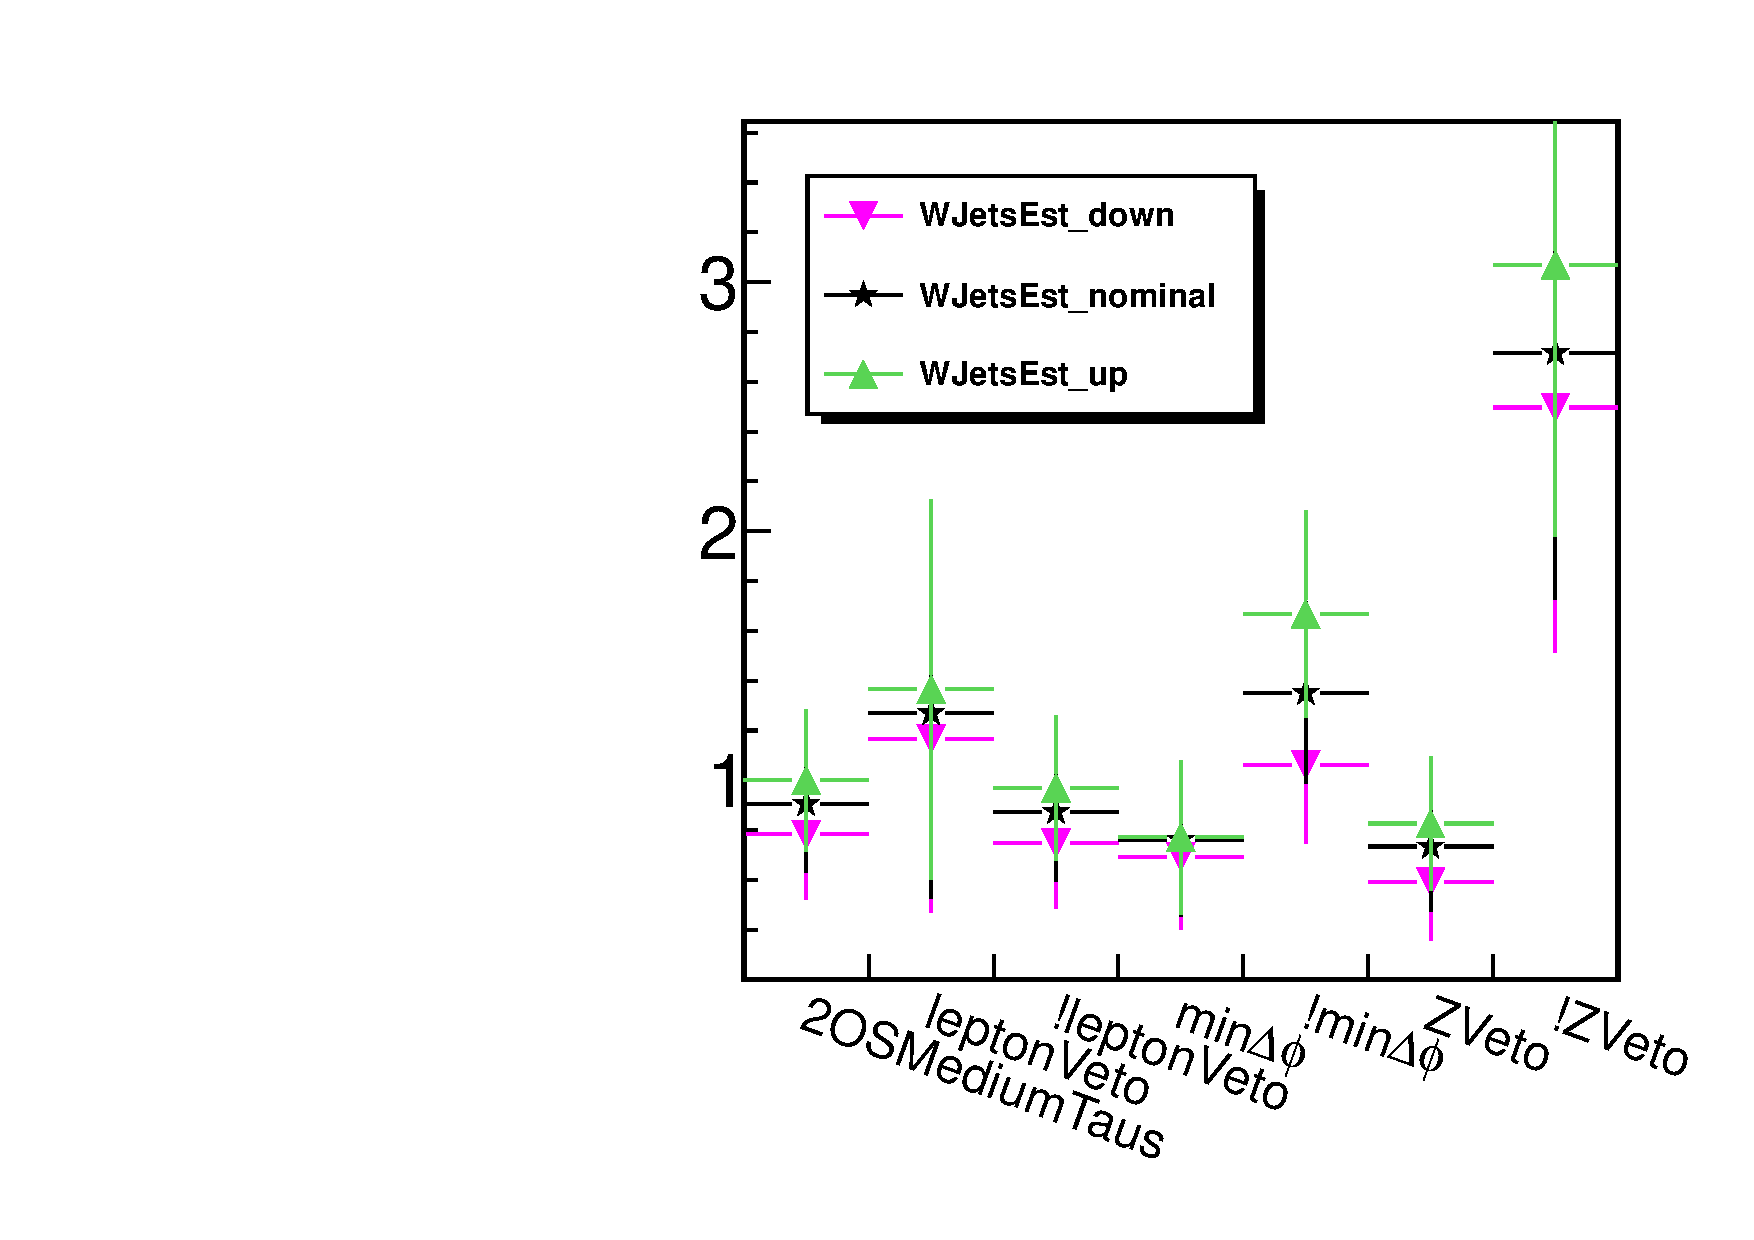
\includegraphics[angle=0,scale=0.35]{TauTauFigs/WJets_bin1.pdf}
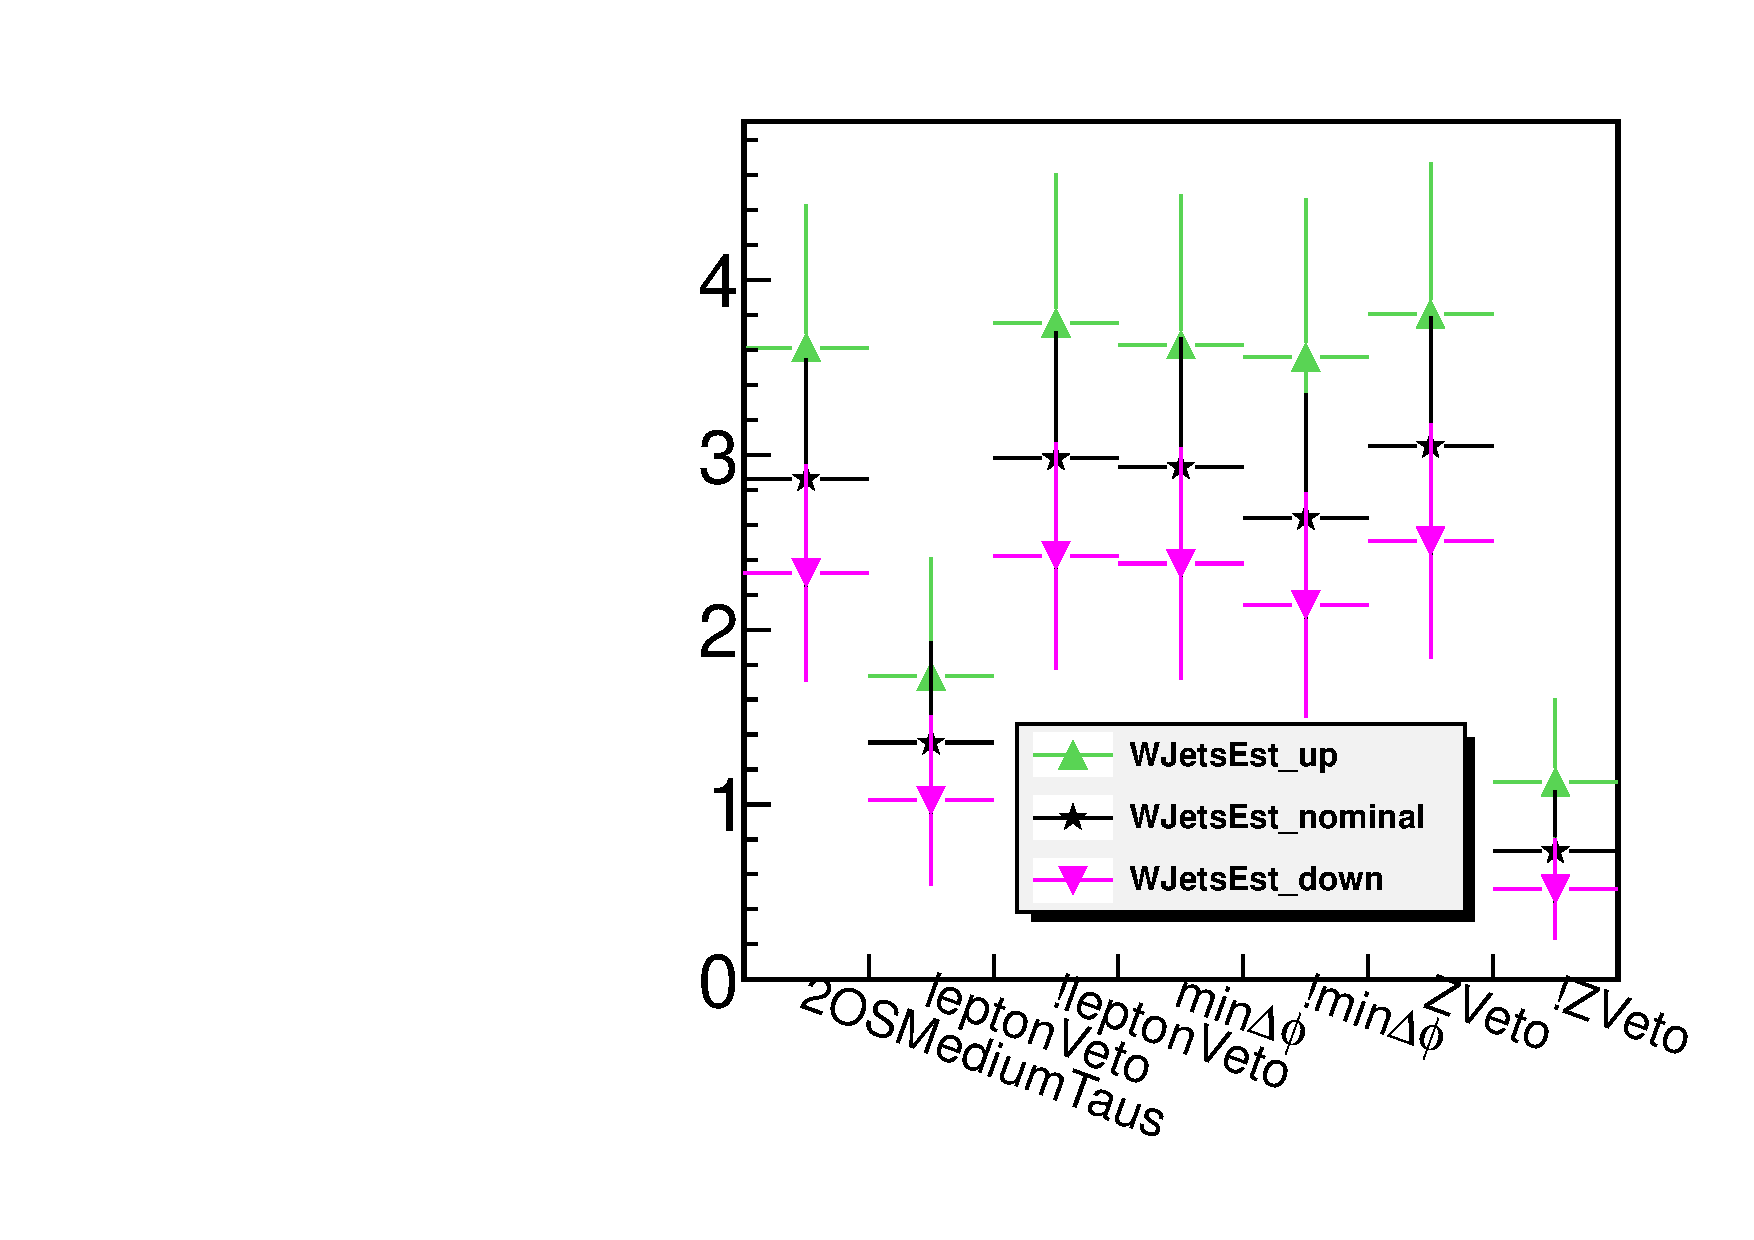
\includegraphics[angle=0,scale=0.35]{TauTauFigs/WJets_binII.pdf}\\
\caption{The distribution of the final estimated \wjets events in \binone (\bintwo) is shown in black in the left (right) plot. 
 The first bin of the histogram corresponds to the sample of events passing the baseline selection cuts. 
The next six bins correspond to the samples where passing and failing the 
list of cuts mentioned in the text, respectively. Also shown are the estimated \wjets events in up and down scaled samples to evaluate the systematics.}
\label{fig:wjets_1}
\end{figure}

Each of the three graphs in both plots in figure~\ref{fig:wjets_1} are fitted with a pol0 function. The results are summarized in table~\ref{tbl:fitpars}.
\begin{table}[!Hhtb]
\begin{center}
\caption{The fit parameters obtained from \wjets estimation results in nominal, up and down scaled samples.}
\begin{tabular}{lcc}
\hline\hline
& \binone &\bintwo \\
  & Fit Parameters (pol0) & Fit Parameters (pol0) \\
\hline\hline
down & 0.79 $\pm$ 0.12 & 1.37 $\pm$ 0.19\\
nominal & 0.93 $\pm$ 0.13 &  1.81 $\pm$ 0.22\\
up & 1.02 $\pm$ 0.13 & 2.52 $\pm$ 0.27\\ 
\hline\hline
\end{tabular}
\label{tbl:fitpars}
\end{center}
\end{table}

The systematic that can be assigned in either of the two search regions is the maximum variation of the up and down central values with 
respect to the nominal one. 

\subsubsection{MC validation for Wjets}
To verify that the MC has a good description of the \wjets events and it can be trusted for both shape and normalization, a data/MC comparison 
is done in a \wjets enriched sample. To enrich the sample, \muTau selection is done with the following modifications:
\begin{itemize}
\item $\mu$ and \Tau are same sign.
\item B-tagged jets with CSVL are vetoed.
\item \Tau isolation changed from Tight to Loose.
\item \tauMT cut is removed.
\end{itemize}
Figure \ref{fig:WValidation} 
\begin{figure}[!Hhtb]
\centering
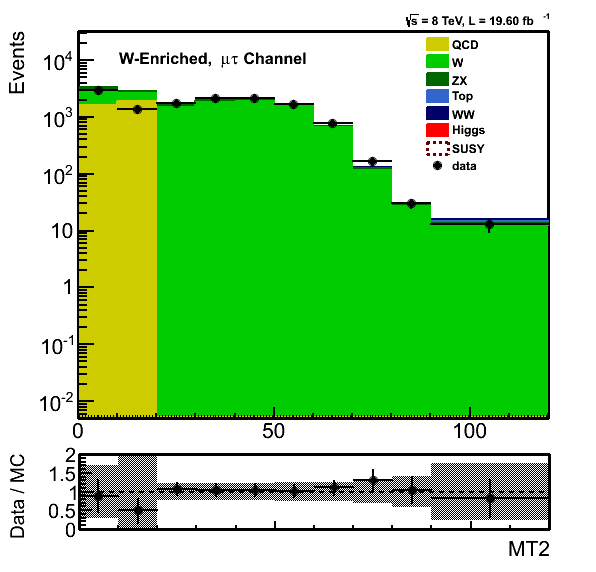
\includegraphics[angle=0,scale=0.375]{TauTauFigs/MT2_WValidation.png}
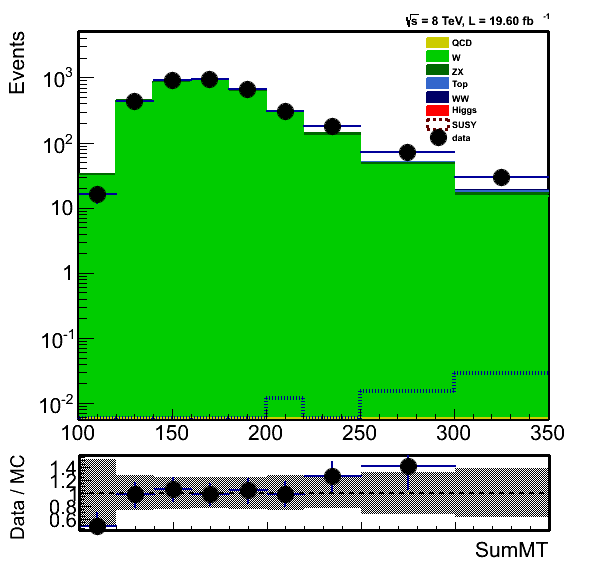
\includegraphics[angle=0,scale=0.375]{TauTauFigs/summt_WValidationBinII_reBinned.png}\\
\caption{Left (Right): The \mttwo ($\SumMT$) distribution in the W-enriched region. Data and MC agree in both shape and normalization within the uncertainties.}
\label{fig:WValidation}
\end{figure}
shows the distributions of the $\mttwo$ and $\SumMT$ for the selected events. For the left (right) plot, the range 40 $<\mttwo<$ 60 \GeV (120 $<\SumMT<$ 220 \GeV) is used to find the normalization factor of the \wjets sample. In the mentioned range of the left (right) plot, it is found that more than 90\% (93\%) of the MC events are from the \wjets sample. 
To extract a normalization factor for the \wjets sample from each of the two plots, non-W MC events are subtracted from the data in the same range 
and the result is compared with the MC prediction for the \wjets in that range. From the left plot, the normalization factor is 
found to be 1.05 $\pm$ 0.13 while from the right plot, one can get a normalization factor of 1.02 $\pm$ 0.09, which ,in both cases, 
is compatible with 1 within the uncertainties. To evaluate the uncertainty, 
all of the statistical uncertainties on data and MC are considered plus 25\% systematic uncertainty on the MC samples.

To validate the shape of the \wjets sample in the left plot, we compare the ratio of events with \mttwo $>$ 90 \GeV and  \mttwo $>$ 40 \GeV in data and MC.
While for the shape validation in the right plot, the efficiency of cutting on $\SumMT>$ 250 \GeV in data and MC is compared. 
The procedures to find the \wjets in data and consider the uncertainties are exactly the same as the procedures for extracting the normalization  
factor. For the left (right) plot, this ratio is found to be 0.00213 $\pm$ 0.00086 (0.0277 $\pm$ 0.0032) in data and  0.0029 $\pm$ 0.0019 (0.0185 $\pm$ 0.0042) in MC. 
 To take into account the difference between the data and MC values, the MC prediction in each of the two search regions is corrected by the ratio of the two values and its uncertainty is also taken into account. % which is about 70\%. 
This uncertainty  is added to other systematic uncertainties of the estimation in quadrature.
A summary of the estimated \wjets events can be found in table~\ref{tbl:Wbkg}. 
\begin{table}[!Hhtb]
\begin{center}
\caption{The \wjets estimation results in both search regions. The systematics due to the fit comes from the maximum 
variation of the estimation found from up and down scaled samples with respect to the nominal one. The ``sys. shape''
takes into account the difference between the shape of the search variable distribution in data and Monte Carlo.}
\begin{tabular}{lc}
\hline\hline
Signal Region & \wjets Estimation Results\\
\hline
\tauTau \binone & 0.69 $\pm$ 0.13 (stat.) $\pm$ 0.14 (sys. fit) $\pm$ 0.52 (sys. shape)\\
\tauTau \bintwo & 2.70 $\pm$ 0.22 (stat.) $\pm$ 0.71 (sys. fit) $\pm$ 0.68 (sys. shape)\\
\hline\hline 
\end{tabular}
\label{tbl:Wbkg}
\end{center}
\end{table}

